\chapter{INTRODUCTION}
Since the seminal report by \citet{Reid1910}, it has been recognized that earthquakes are caused by the sudden release of elastic strain energy that has gradually accumulated over time along tectonic plate boundaries. If one assumes that strain is accumulating at a constant rate, then modern-day geodetic observations of tectonic deformation can be used to infer parameters that are fundamentally important for assessing seismic hazard, such as long term fault slip rates \citep[e.g.,][]{Savage1973,Meade2005}. Indeed, such an assumption has been made in constraining the latest, and most authoritative, seismic hazard model for California, UCERF3 \citep{Field2014}. However, plate tectonics is a more dynamic process, and we can better understand earthquakes, as well as the Earth itself, by considering the time-dependence of tectonic deformation. 

Consider a simple model where an elastic layer, representing the lithosphere, is overlying a viscous substrate, representing the asthenosphere (Figure \ref{intro:fig:1}). Immediately after an earthquake, stresses will be perturbed in the substrate and ground deformation should be most rapid while these coseismic stresses are being viscously relaxed \citep{Nur1974,Savage1978}. Shear stresses will also be increased on the fault surrounding the area that ruptured in the earthquake. These heightened shear stresses can be released seismically through aftershocks or aseismically through afterslip \citep{Marone1991}. Observations of ground deformation resulting from these postseismic processes, termed postseismic deformation, can then be used to constrain the strength of the asthenosphere and the frictional properties of faults. Both of which can then be used to better understand how elastic strain energy is accumulating on faults. 

\begin{figure}
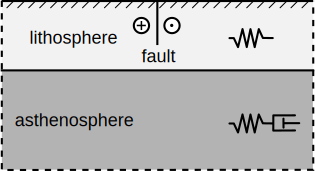
\includegraphics{schematic}
\caption
[Schematic of a postseismic deformation model]
{Schematic of a postseismic deformation model. A strike-slip fault is embedded in an elastic layer which overlies a viscoelastic substrate. This schematic is modeled after \citep{Savage1978}.}
\label{intro:fig:1}
\end{figure}

Some of the first observations of postseismic deformation came from
leveling and triangulation surveys
\citep[e.g,][]{Kanamori1973,Thatcher1975}. These geodetic techniques
detected deformation to within an accuracy of a few centimeters and at
sampling intervals on the order of years. With the advent of space
geodetic techniques, such as Global Navigation Satellite Systems
(GNSS)\footnote{The terms ``GNSS" and ``GPS" (Global Positioning
System) will be used synonymously in this dissertation, although GPS
is specifically operated by the United States and GNSS is a more
generic term.}, geodetic observations have become more precise and
have achieved higher sampling rates. Furthermore, in the past decade a
dense network of geodetic instruments, consisting of GNSS stations and
borehole strain meters, have been installed along the Western United
States as part of the Plate Boundary Observatory (PBO). This
unprecedented data coverage and data quality has improved our ability
to resolve postseismic deformation and has lead to the recent
discovery of slow slip events along the Cascadia subduction zone
\citep{Dragert2001}. Slow slip events occur deep on the subduction
zone and they tend to migrate stresses up onto the seismogenic portion
of the fault. Slow slip events thus pose a serious risk of triggering
megathrust earthquakes and should be factored in to assessments of
seismic hazard.

In this dissertation I study transient deformation associated with
tectonic processes, such as postseismic deformation and slow slip
events. The immediate objective of this dissertation is to detect
transient deformation and better understand the mechanisms causing it.
The broader motivation for my research is to improve our understanding
of earthquakes and seismic hazard. The chapters of this dissertation
can be separated into model-based and data-based analysis. Chapters 2,
3, and 4 are model-based, where I discuss how physical models of
tectonic processes can be constrained by observable transient
deformation. Chapters 5, 6, and 7 are data-based, where I am mostly
focused on assessing the noise in geodetic data and detecting
transient geophysical signal.

\section{Outline}
Chapter 2 presents a theoretical discussion on what can and cannot be
said about the strength of the lithosphere based on interseismic
deformation. Interseismic deformation is considered to be deformation
over the entire earthquake cycle (100s of years), whereas the
postseismic deformation mentioned above tends to refer to deformation
in the days to years following an earthquake. Both types of
deformation exhibit transients, although interseismic transients is
over a much longer timescale. Several studies have used interseismic
deformation to infer the strength of the crust and upper mantle. These
studies have almost unanimously concluded that the crust is relatively
strong compared to the upper mantle \citep{Thatcher2008}. In this
chapter I urge caution when interpreting the results of such studies,
because I demonstrate that their methodology is inherently biased
towards overestimating and underestimated the strength of the crust
and upper mantle, respectively. The bias results from the commonly
simplifying employed assumption that the viscosities are uniform
within the lower crust and upper mantle.

Chapter 3 and 4 focus on modeling postseismic deformation, where my
goal is to infer the lithospheric viscosity and distribution of
afterslip from observable postseismic deformation. Such an inverse
problem tends to be computationally intractable because there are many
unknown parameters being estimated. Additionally, the forward problem
is nonlinear with respect to the unknown parameters, and it must be
solved with numerical methods. In Chapter 3 we present a approximation
for the postseismic deformation forward problem that can be used to
make the inverse problem computationally tractable. We demonstrate
that our method is able to accurately identify the stength of the
lithospheric from postseismic deformation even while afterslip is
obscuring the signal from viscous relaxation. Chapter 4 is an
application of this method, where I analyze five years of postseismic
deformation following the 2010 El Mayor-Cucapah earthquake in Baja
California. One of my major findings in Chapter 4 is that an
accelerated rate of deformation can be observed several hundred
kilometers away for the earthquake epicenter. While this far reaching
deformation is not immediately recognizable from the raw GPS data, I
am able to observe a coherent signal after using a Kalman filtering
strategy that I developed and describe in this chapter. I then analyze
this postseismic signal to determine the physical mechanism causing
it. I find that the far field deformation is best described by a
Burgers rheology upper mantle with a transient viscosity of about
$10^{18}$ Pa$\cdot$s. My finding that the mantle is best described
with a Burgers rheology, rather than the more commonly employed
Maxwell rheology, is more consistent with mantle viscosities
determined in other types of geophysical studies
\citep[e.g.,][]{Crittenden1967,Bills1987}.

Chapter 5 is on quantifying noise in geodetic time series.  While this
chapter does not directly discuss transient deformation, it is
necessary to accurately quantify the noise in geodetic data before any
transient signal can be identified. We discuss a bias in a commonly
used method for quantifying noise in geodetic data. This bias tends to
underestimate the amplitude of noise, which then results in
underestimated uncertainties for any geophysical parameters derived
from the data. We demonstrate that the Restricted Maximum Likelihood
(REML) technique, which was first introduced by \citet{Patterson1971},
can be used as an alternative unbiased method for characterizing noise
in geodetic data.

In Chapter 6 we discuss a non-parametric method for detecting
transient deformation, specifically transient strain, in GNSS data.
Existing transient detection methods tend to assume a parametric form
for the underlying signal being detected \citep[e.g.,][]{Ohtani2010},
and an improperly chosen parameterization can bias the results. Our
method for detecting transient deformation uses Gaussian process
regression, where we assume a stochastic prior model for the
underlying signal. As opposed to a subjectively chosen parametric
model, our stochastic prior model can be objectively chosen using
maximum likelihood techniques, such as the REML method discussed in
Chapter 5. We demonstrate our method by applying it to GNSS data from
the Pacific Northwest, where we detect transient strain from slow slip
events. We verify the accuracy of our detection method by comparing
our inferred geophysical signal to observations of seismic tremor,
which are known to coincide with slow slip events.

Chapter 7 is a discussion on borehole strain meters (BSMs) and their
ability to record strain from slow slip events. The PBO contains 82
BSMs; however, the data recorded by these instruments is seldom used.
This is perhaps because it is unclear whether BSM data, which
describes strains over a 8.7 centimeter baseline, are representative
of regional tectonic strains. We address this question by comparing
GNSS derived strains, described in Chapter 6, to the strains recorded
at BSMs. We find that only two BSMs record data that is consistent
with the regional strains derived from GNSS data. A third station can
be made consistent with the GNSS derived strains if we assume that it
is misoriented.

Finally, in Chapter 8 we discuss future research directions and
provide concluding remarks.

\section{Publications from this dissertation}
This dissertation consists of three published manuscripts, two
manuscripts that are currently in review, and one manuscript that is
in preparation. The published and submitted manuscripts are listed
below.

\begin{itemize}
\item{Hines, T. T., and Hetland, E. A. (2013). Bias in estimates of lithosphere viscosity from interseismic deformation. Geophysical Research Letters, 40, 4260--4265, doi:10.1002/grl.50839. \textbf{Chapter 2}}  
\item{Hines, T. T., and Hetland, E. A. (2015). Rapid and simultaneous estimation of fault slip and heterogeneous lithospheric viscosity from post-seismic deformation. Geophysical Journal International, 204, 569–582, doi:10.1093/gji/ggv477. \textbf{Chapter 3}} 
\item{Hines, T. T., and Hetland, E. A. (2016). Rheologic constraints on the upper mantle from five years of postseismic deformation following the El Mayor-Cucapah earthquake. Journal of Geophysical Research: Solid Earth, 121, doi:10.1002/2016JB013114. \textbf{Chapter 4}}
\item{Hines, T. T., and Hetland, E. A. (2017). Unbiased characterization of noise in geodetic data. submitted to Journal of Geodesy \textbf{Chapter 5}}
\item{Hines, T. T., and Hetland, E. A. (2017). Revealing transient strain in geodetic data with Gaussian process regression. submitted to Geophysical Journal International \textbf{Chapter 6}} 
\end{itemize}
